% Options for packages loaded elsewhere
% Options for packages loaded elsewhere
\PassOptionsToPackage{unicode}{hyperref}
\PassOptionsToPackage{hyphens}{url}
\PassOptionsToPackage{dvipsnames,svgnames,x11names}{xcolor}
%
\documentclass[
  letterpaper,
  DIV=11,
  numbers=noendperiod]{scrreprt}
\usepackage{xcolor}
\usepackage{amsmath,amssymb}
\setcounter{secnumdepth}{5}
\usepackage{iftex}
\ifPDFTeX
  \usepackage[T1]{fontenc}
  \usepackage[utf8]{inputenc}
  \usepackage{textcomp} % provide euro and other symbols
\else % if luatex or xetex
  \usepackage{unicode-math} % this also loads fontspec
  \defaultfontfeatures{Scale=MatchLowercase}
  \defaultfontfeatures[\rmfamily]{Ligatures=TeX,Scale=1}
\fi
\usepackage{lmodern}
\ifPDFTeX\else
  % xetex/luatex font selection
\fi
% Use upquote if available, for straight quotes in verbatim environments
\IfFileExists{upquote.sty}{\usepackage{upquote}}{}
\IfFileExists{microtype.sty}{% use microtype if available
  \usepackage[]{microtype}
  \UseMicrotypeSet[protrusion]{basicmath} % disable protrusion for tt fonts
}{}
\makeatletter
\@ifundefined{KOMAClassName}{% if non-KOMA class
  \IfFileExists{parskip.sty}{%
    \usepackage{parskip}
  }{% else
    \setlength{\parindent}{0pt}
    \setlength{\parskip}{6pt plus 2pt minus 1pt}}
}{% if KOMA class
  \KOMAoptions{parskip=half}}
\makeatother
% Make \paragraph and \subparagraph free-standing
\makeatletter
\ifx\paragraph\undefined\else
  \let\oldparagraph\paragraph
  \renewcommand{\paragraph}{
    \@ifstar
      \xxxParagraphStar
      \xxxParagraphNoStar
  }
  \newcommand{\xxxParagraphStar}[1]{\oldparagraph*{#1}\mbox{}}
  \newcommand{\xxxParagraphNoStar}[1]{\oldparagraph{#1}\mbox{}}
\fi
\ifx\subparagraph\undefined\else
  \let\oldsubparagraph\subparagraph
  \renewcommand{\subparagraph}{
    \@ifstar
      \xxxSubParagraphStar
      \xxxSubParagraphNoStar
  }
  \newcommand{\xxxSubParagraphStar}[1]{\oldsubparagraph*{#1}\mbox{}}
  \newcommand{\xxxSubParagraphNoStar}[1]{\oldsubparagraph{#1}\mbox{}}
\fi
\makeatother


\usepackage{longtable,booktabs,array}
\usepackage{calc} % for calculating minipage widths
% Correct order of tables after \paragraph or \subparagraph
\usepackage{etoolbox}
\makeatletter
\patchcmd\longtable{\par}{\if@noskipsec\mbox{}\fi\par}{}{}
\makeatother
% Allow footnotes in longtable head/foot
\IfFileExists{footnotehyper.sty}{\usepackage{footnotehyper}}{\usepackage{footnote}}
\makesavenoteenv{longtable}
\usepackage{graphicx}
\makeatletter
\newsavebox\pandoc@box
\newcommand*\pandocbounded[1]{% scales image to fit in text height/width
  \sbox\pandoc@box{#1}%
  \Gscale@div\@tempa{\textheight}{\dimexpr\ht\pandoc@box+\dp\pandoc@box\relax}%
  \Gscale@div\@tempb{\linewidth}{\wd\pandoc@box}%
  \ifdim\@tempb\p@<\@tempa\p@\let\@tempa\@tempb\fi% select the smaller of both
  \ifdim\@tempa\p@<\p@\scalebox{\@tempa}{\usebox\pandoc@box}%
  \else\usebox{\pandoc@box}%
  \fi%
}
% Set default figure placement to htbp
\def\fps@figure{htbp}
\makeatother





\setlength{\emergencystretch}{3em} % prevent overfull lines

\providecommand{\tightlist}{%
  \setlength{\itemsep}{0pt}\setlength{\parskip}{0pt}}



 


\KOMAoption{captions}{tableheading}
\makeatletter
\@ifpackageloaded{bookmark}{}{\usepackage{bookmark}}
\makeatother
\makeatletter
\@ifpackageloaded{caption}{}{\usepackage{caption}}
\AtBeginDocument{%
\ifdefined\contentsname
  \renewcommand*\contentsname{Table of contents}
\else
  \newcommand\contentsname{Table of contents}
\fi
\ifdefined\listfigurename
  \renewcommand*\listfigurename{List of Figures}
\else
  \newcommand\listfigurename{List of Figures}
\fi
\ifdefined\listtablename
  \renewcommand*\listtablename{List of Tables}
\else
  \newcommand\listtablename{List of Tables}
\fi
\ifdefined\figurename
  \renewcommand*\figurename{Figure}
\else
  \newcommand\figurename{Figure}
\fi
\ifdefined\tablename
  \renewcommand*\tablename{Table}
\else
  \newcommand\tablename{Table}
\fi
}
\@ifpackageloaded{float}{}{\usepackage{float}}
\floatstyle{ruled}
\@ifundefined{c@chapter}{\newfloat{codelisting}{h}{lop}}{\newfloat{codelisting}{h}{lop}[chapter]}
\floatname{codelisting}{Listing}
\newcommand*\listoflistings{\listof{codelisting}{List of Listings}}
\makeatother
\makeatletter
\makeatother
\makeatletter
\@ifpackageloaded{caption}{}{\usepackage{caption}}
\@ifpackageloaded{subcaption}{}{\usepackage{subcaption}}
\makeatother
\usepackage{bookmark}
\IfFileExists{xurl.sty}{\usepackage{xurl}}{} % add URL line breaks if available
\urlstyle{same}
\hypersetup{
  pdftitle={Daniel W. G.},
  pdfauthor={18224114 Daniel Wicaksana Godjali},
  colorlinks=true,
  linkcolor={blue},
  filecolor={Maroon},
  citecolor={Blue},
  urlcolor={Blue},
  pdfcreator={LaTeX via pandoc}}


\title{Daniel W. G.}
\usepackage{etoolbox}
\makeatletter
\providecommand{\subtitle}[1]{% add subtitle to \maketitle
  \apptocmd{\@title}{\par {\large #1 \par}}{}{}
}
\makeatother
\subtitle{Portfolio Asesmen II-2100 KIPP}
\author{18224114 Daniel Wicaksana Godjali}
\date{2027-06-10}
\begin{document}
\maketitle

\renewcommand*\contentsname{Table of contents}
{
\hypersetup{linkcolor=}
\setcounter{tocdepth}{2}
\tableofcontents
}

\bookmarksetup{startatroot}

\chapter*{Pendahuluan}\label{pendahuluan}
\addcontentsline{toc}{chapter}{Pendahuluan}

\markboth{Pendahuluan}{Pendahuluan}

\textbf{Perkenalan Singkat}

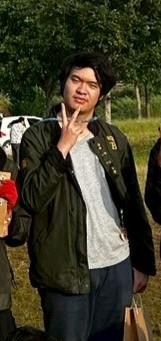
\includegraphics[width=0.5\linewidth,height=\textheight,keepaspectratio]{images/LANTIK.jpg}

Daniel Wicaksana Godjali adalah seorang mahasiswa Sekolah Teknik Elektro
dan Informatika - Komputasi angkatan 2024. Lahir di Bandung, pada
tanggal 7 Mei 2006. Daniel merupakan anak ke-2 dari 2 bersaudara.

Laman ini adalah pemaparan dari rangkaian Tugas Ujian II-2100. Berisi
tentang cerita-cerita diri saya, suara dan rasa saya ke orang-orang yang
saya hargai, Pendapat saya ke beragam hal, dan lain-lain.

Semoga apa yang saya kemukakan di situs ini bisa tersampaikan dan
bermanfaat bagi pembaca (bila ada). Silahkan mengunjungi navbar di sisi
kiri untuk melanjutkan.

\bookmarksetup{startatroot}

\chapter{UTS-1 All About Me}\label{uts-1-all-about-me}

\section{\texorpdfstring{\textbf{Pembuka}}{Pembuka}}\label{pembuka}

``Fun'' Facts diri saya:

\textbf{1. Saya buta warna parsial}

Lebih tepatnya buta warna merah-hijau. Atau istilah ilmiahnya itu
\emph{Deuteranopia}. Saya sering diketawain teman-teman saya dari dulu
gara-gara tidak bisa membedakan warna-warna seperti hijau-cokelat,
pink-abu, abu-hijau, hijau-biru, pink-ungu, dan lain-lain.

\textbf{2. Semua keluarga (utama) saya adalah alumni ITB}

Saya bagian dari STEI-K, Kakak saya bagian dari FSRD, Ibu dan Kakek
bagian dari SAPPK, Ayah bagian dari FITB, dan Nenek bagian dari SF.

\textbf{3. Saya satu-satunya di keluarga yang tidak menggunakan
kacamata}

Semua dari keluarga saya memiliki kelainan penglihatan (termasuk saya).
Bedanya adalah saya jarak penglihatannya masih normal. Tapi mereka semua
perlu kacamata yang ``angka''-nya lumayan besar. Semoga tidak berubah,
karena saya tidak begitu suka memakai kacamata.

\section{\texorpdfstring{\textbf{Sejarah Diri
Singkat}}{Sejarah Diri Singkat}}\label{sejarah-diri-singkat}

Saya lahir di Bandung, 7 Mei 2006. Saya semenjak dahulu diajarkan oleh
keluargaku untuk berbaik hati, berbagi, dan bersabar. Namun karena saya
kurang diajarkan cara mengendalikan emosi dan amarah, saya menjadi anak
yang sensi selama masa kecil. Saya pada umur 4 dimasukan ke Play-Group
``Santa Angela'' dimana saya akan disana hingga SMA. Pada masa TK dan
SD, saya dikenal sebagai anak yang cengeng karena sering menangis
setelah diledek-ledek oleh teman. Untungnya pada saat saya masuk SMP
sudah mengurang. Pada masa saya kelas 8 hingga 11 ada wabah covid
sehingga semua aktivitas akademik dijalankan secara daring. Akibatnya
pertemanan saya tidak meluas dan itu-itu saja. Dan di pertengahan
semester ganjil kelas 11, saya harus pindah ke homeschooling di sekolah
``Pewaris Bangsa'' akibat setelah pelajaran dijalankan secara tatap muka
kembali saya mengalami masalah kesehatan berat. Meskipun demikian, saya
masih dapat lolos masuk ke STEI-K ITB melalui jalur mandiri.

\section{\texorpdfstring{\textbf{Hobi \&
Minat-Bakat}}{Hobi \& Minat-Bakat}}\label{hobi-minat-bakat}

Hobi saya adalah bermain game komputer, membaca buku, bermain catur, dan
bermain badminton. Saya senang bermain game Dulu saya sering banget main
game sampai orang tua saya lelah menegur saya. Saya sering membaca novel
terutama genre mystery dan fantasy. Saya pernah mengikuti
ekstrakurikuler catur dan badminton di SMP dan SD. Saya senang kedua
kegiatan tersebut. Namun sayangnya saya kurang memiliki waktu untuk
melakukan hal-hal tersebut akhir-akhir ini.

Minat saya adalah dalam bidang back-end, cybersec, dan
software-engineering. Saya sudah mendalami programming semenjak sekitar
kelas 4 SD. Dan saya terus mendalaminya hingga sekarang. Namun di masa
SMA saya kurang mendalami karena sibuk untuk belajar ujian-ujian yang
banyak, khususnya penerimaan mahasiswa baru. Namun semenjak di STEI-K
saya semakin semangat mendalami kembali dunia programming.

\section{\texorpdfstring{\textbf{Personality}}{Personality}}\label{personality}

Karena sering-sering disuruh masukin MBTI untuk perkenalan-perkenalan,
saya melakukan tesnya dan mendapatakn \textbf{INTJ}. Dan saya lumayan
setuju dengan apa yang disebutkannya dan bahkan stereotip mereka. Saya
adalah introvert yang lebih mudah lelah saat bersosialisasi dan
berkomunikasi bahkan ke keluarga sendiri. Saya memiliki imaginasi yang
luas dan seringkali melamun di kelas karena day-dreaming bila materinya
membosankan. Selain itu saya sering banget over-thinking apalagi dalam
konteks sosial. Saya membayangkan bila orang bertanya x ke saya saya
jawabnya apa dan apabila saya jawab y, apa respon dari orang tersebut
(mungkin itu kenapa saya lelah banget saat bersosialisasi). Saya selama
masa kecil memang terlalu sensi, tapi sekarang saya kurang bisa peka
terhadap keadaan emosi orang lain (dense/insensitive kata orang meh)
karena saya fokus dengan logika dan pikiran aja. Dan saya juga suka
hal-hal yang teratur. Saya hanya peduli kerapihan dari hal-hal yang
menurut saya penting saja. Tapi bila saya anggap kurang penting saya
jujur seringkali abaikan saja karena antara: 1. Beneran gak peduli, 2.
Saya anggep kurang penting, atau 3. Pasrah atas keadaan dan merasa
terlalu repot untuk saya organisir dan masuk mode priority management.

\section{\texorpdfstring{\textbf{Values}}{Values}}\label{values}

Ada beberapa nilai penting yang saya pegang selama hidup saya:

\textbf{1. Selalu bersikap adil ke semua orang}

Sebagai orang yang terundungi di masa lalu dan diabaikan oleh orangtua
dan guru mengenainya, saya mengetahui apa rasanya diperlakukan tidak
adil oleh orang lain. Maka itu saya akan selalu bersikap adil ke orang
lain dan tidak memandang semata-mata saja.

\textbf{2. Selalu berbaik hati dan sopan ke orang lain hingga mereka
tidak lagi layak menerimanya}

Melanjuti dari nilai sebelumnya, saya memiliki pandangan bahwa semua
orang memiliki hak untuk dihormati, dihargai, dan diperlakukan dengan
baik. Namun saya juga mengerti bahwa tidak semua orang bisa melakukan
hal tersebut ke orang lain dan tidak semua orang layak untuk
diperlakukan tersebut. Maka tanpa alasan yang jelas, semua orang akan
saya hormati, harga, dan perlakukan dengan baik dan sopan hingga ada
alasan yang tidak dapat diabaikan untuk tidak lagi memperlakukan orang
dengan baik. (ini maksudnya jangan gak sopan atau jahat ke orang lain
tanpa alasan jelas dan masuk akal, jangan gara-gara lagi bad mood
tiba-tiba crash out ke orang lain sambil menghina dan memaki)

\textbf{3. Lakukan yang terbaik dan tetaplah maju kedepan apapun
hasilnya}

Saya memandang bahwa bila mendapatkan kesusahan, kegagalan, dan
kepedihan, menangis, kesal, marah, dan lainnya tidak akan membantu kita.
Bila merasa ingin menyerah, saya mengingat lagi bahwa hidup hanya sekali
saja dan kita hanya bisa menjalaninya dengan sebaik mungkin. Maka itu
saya percaya bahwa meskipun kegagalan menunggu, jalanilah hingga
akhirnya. Setidaknya jalanilah hidup anda hingga akhir.

\bookmarksetup{startatroot}

\chapter{UTS-2 My Songs for You}\label{uts-2-my-songs-for-you}

Lagu ini ditunjukan ke keluarga saya yang telah mendorong dan mendukung
saya hingga diri disaat ini. Lagu ini mencerminkan bagaiman perjalanan
hidup saya hingga saat ini.

Bagaimana saya menjalani hidup saya yang mulai dari kecil hingga
sekarang, bagaimana saya memandang kesulitan kepedihan hidup, dan
bagaimana meskipun tidak sesuai dengan keinginan saya, keluargaku tetap
membantu saya ke masa depan yang lebih baik.

\url{https://www.youtube.com/watch?v=ZuifkacZ0TA}

\textbf{{[}Verse 1{]}}

One, two

One, two, three, four

We're swaying on horseback, the hills are green

And the birdies sing, and roses are pink

Experience I never had, I'm so happy

Happy to just be part of your story

\textbf{{[}Pre-Chorus 1{]}}

After you, I follow

After you, I follow

The world you show me broaden my horizon

\textbf{{[}Chorus 1{]}}

Forever my hero

Forever my hero

I am your biggest fan

I am your biggest fan

\textbf{{[}Verse 2{]}}

Merry-go-round in a circle I run

It's so much fun leaving reality behind

One, two

One, two, three, four

I fall down the horseback with my cripple legs

And then it starts to rain, showing me it's all fake

Raindrops wash down the facade hills are painted

Birdies are robotic, roses are made of clay

\textbf{{[}Pre-Chorus 2{]}}

Excitement that I feel

Excitement that I feel

Return them to the shelf 'cause now I understand

\textbf{{[}Chorus 2{]}}

Heroes cannot be real

Heroes cannot be real

I wasn't who I am

I don't know who I am

\textbf{{[}Bridge 1/Breakdown{]}}

Who am I?

Who am I?

Who am I?

Here we go another lap, prizes to claim

Here's a dream for you

Here's a dream for me

Golden tickets in my bag stay unchanged

Don't you love the thrill of the chase?

Just let me be your fan, I wanna be your fan

I'm still your biggest fan

\textbf{{[}Bridge 2/Reflection{]}}

Why is it that some were given the role of villain?

The moment they were released into this system?

\textbf{{[}Verse 3/Outro{]}}

One, two

One, two, three, four

Stand up, gallop on

Nothing can be done by feeling so sorry for myself

Hero on a plastic horse

Fighting like it's real with a cardboard sword

I know successful or not, I am who I am

I am my biggest fan

I am my biggest fan

I am my enemy and my friend

Hero gonna prove my version of justice

Is more just than yours

Uno remaining on this stage, I am the only one

I am my biggest fan

I am my biggest fan

I am my enemy and my friend

\bookmarksetup{startatroot}

\chapter{UTS-3 My Stories for You}\label{uts-3-my-stories-for-you}

\textbf{Sebuah cuplikan dari hidup saya}

Saya sudah bercerita tentang sejarah hidup saya secara singkat di page
\hyperref[uts-1-all-about-me]{All About Me}. Disana saya sebut bahwa
saya adalah anak yang cengeng karena banyak teman kelas yang suka
mengejek-ejek saya. Setiap kali saya mencoba bercurah hati ke orangtua
ataupun guru, mereka hanya menganggap remeh dan tidak penting. Saya
tidak tahu cara menghandal teman yang meledek saya tersebut. Saya
diejek-ejek terus menerus hingga saya tidak tahan lagi dan mulai melawan
secara fisik. Hal tersebut memang mengurangi ejekan terhadap saya
(meskipun tidak banyak). Namun akibatnya saya semakin tidak memiliki
teman. Saya juga tidak dapat mempercayai guru lagi akibat ada insiden di
kelas 5 dimana guru wali kelas saya menganggap saya tidak sopan dan
menarik saya pada leher ke ruang Bimbingan Konseling di Lantai 1 dari
Lantai 2. Hal tersebut menghancurkan kemungkinan saya berteman dengan
seorang guru lainnya di masa depan.

Untungnya saya selama SMP ada grup teman yang bisa saya ajak bermain dan
ngobrol. Grup kami mulai terbentuk di akhir SD/awal SMP. Kami bermain
game bersama, mengerjakan tugas bersama, dan juga nongkrong dan
jalan-jalan bersama. Saya merasa nyaman di lingkungan tersebut karena
bisa dengan bebas tertawa, bersengang-senang, dan menunjukan diri saya.
Namun di akhir kelas 9, ``leader'' grup teman tersebut mulai
meng-ghosting saya dan beberapa teman lainnya karena alasan entah-apa.
Orang yang meng-ghosting ini saya kira sangat dekat dengannya, kami
selalu ngobrol setelah kelas berakhir ataupun saat istirahat, saling
belajar, dan sangat sering bermain bersama. Maka itu saya lumayan kaget
dan bingung mengapa Ia tidak lagi menjawab saya (ini pada masa covid).
Saya mencoba mengkontak dan meminta maaf bila saya menyebutkan suatu hal
yang salah, tapi tidak ada suara balasan apa-apa, hanya kesunyian.

Setelah itu saya merasa terkucilkan kembali dan mulai depresi parah
(Menyalahkan diri sendiri, Tidak merawat diri sendiri, Membenci diri,
dan juga Keinginan Bunuh Diri). Saya pada masa tersebut merasa bahwa
saya memang orang yang tidak pantas mendapat teman ataupun orang yang
mempedulikan saya. Saya merasa semua hal buruk yang terjadi di masa lalu
saya memang takdir karena diri saya yang memang tidak pantas merasakan
kebahagiaan karena kejelekan diri saya. Bermacam-macam kalimat seperti
itu muncul di kepala saya. Dan keluarga saya mencoba memberi saya
layanan terapi ini itu namun tidaklah efektif sama-sekali. Dimana saya
sudah merasa kehilangan kepercayaan kepada dunia, keluarga, teman, guru,
diri sendiri, dan juga Tuhan, kondisi saya tidaklah bagus baik secara
fisik ataupun mental. Tapi salah satu teman saya yang ikut di-ghosting
tersebut menghubungi saya karena saya sudah jarang aktif online (ini
masa covid). Saya bercerita sedikit tentang perasaan saya terhadap
di-ghosting tersebut dan Ia mengatakan bahwa bukan hanya saya yang
di-ghosting, memang beberapa orang lain dari grup pertemanan tersebut
ikut di-ghosting. Saya tidak tahu hal ini sebelumnya, saya mengira hanya
diri saya sendiri yang diperlakukan demikian. Ia mengajak saya ke grup
orang yang ter-ghosting juga dan kita pada belajar bersama, bermain
bersama, dan juga jalan-jalan bersama. Kini banyak yang berbeda sekolah
dengan sesama beserta semakin jarang berkumpul karena kesibukan
masing-masing. Meskipun alasan utamanya adalah dendam terhadap orang
yang meng-ghosting tersebut, hubungan kami sangat erat.

Pesan moral dari cerita ini yang ingin saya sampaikan bukanlah untuk
membawa dendam bersama-sama.

Pesan yang ingin saya sampaikan adalah: \textbf{Tidak semua orang itu
baik dan dapat dipercaya. Namun juga tidak semua orang itu jahat dan
tidak dapat dipercaya. Pada malam yang paling gelap sekalipun, pasti
nantinya akan terbitlah pagi. Sekelam dan sepedihnya situasi apapun,
bila kita bisa menjalaninya hingga akhir seberapa lamapun, maka pastinya
akan ada akhir dari kepedihan tersebut.}

\bookmarksetup{startatroot}

\chapter{UTS-4 My SHAPE (Spiritual Gifts, Heart, Abilities, Personality,
Experiences)}\label{uts-4-my-shape-spiritual-gifts-heart-abilities-personality-experiences}

\begin{quote}
\textbf{Tujuan:} Merangkum rancangan diri (charter) agar saya melayani,
berkarya, dan memimpin secara paling selaras dengan karunia dan
pengalaman hidup saya. Dapat langsung ditempel ke halaman \textbf{UTS-4
--- My SHAPE} dan dipakai sebagai acuan aksi 90 hari.
\end{quote}

Sumber \href{StrengthsProfile-Daniel-WG.pdf}{VIA assessment}

\begin{center}\rule{0.5\linewidth}{0.5pt}\end{center}

\section{S --- Spiritual Gifts (Karunia
Rohani)}\label{s-spiritual-gifts-karunia-rohani}

\begin{itemize}
\item
  \textbf{Judgement, Fairness, Prudence:} melakukan keputusan dan
  pertimbangan dengan adil, seksama, teliti, dan terbuka tanpa adanya
  bias.
\item
  \textbf{Honesty:} menjunjung tinggi kejujuran, transparansi, dan
  keterbukaan.
\item
  \textbf{Perseverance:} Pantang menyerah dan menyelesaikan hal yang
  telah dimulai.
\end{itemize}

\begin{center}\rule{0.5\linewidth}{0.5pt}\end{center}

\section{H --- Heart (Minat, Nilai,
Kepedulian)}\label{h-heart-minat-nilai-kepedulian}

\begin{itemize}
\tightlist
\item
  \textbf{JUSTICE}: sebuah hidup yang adil dan tidak menceng serta bebas
  kejahatan dan seimbang
\item
  \textbf{Kreativitas naratif}: novel, cerita, fanfic sebagai media
  ekspresi dunia dan kemungkinan-kemungkinan yang ada
\item
  \textbf{Software Engineering/CyberSecurity/Back-end engineer}
\end{itemize}

\textbf{Masalah yang ingin dipecahkan:} kesenjangan antara
pengetahuan--karakter--aksi; pembelajaran kurang bermakna; layanan
komunitas belum terukur dampaknya.

\begin{center}\rule{0.5\linewidth}{0.5pt}\end{center}

\section{A --- Abilities (Kemampuan
Andal)}\label{a-abilities-kemampuan-andal}

\begin{itemize}
\tightlist
\item
  \textbf{Perancangan sistem} (PSKVE/TISE), \emph{value co‑creation},
  finansial rekayasa, desain instrumen penilaian.
\item
  \textbf{Kurikulum \& pedagogi}: CPMK↔rubrik↔tugas↔bukti; otomasi alur
  kerja (Python/Quarto/GitHub).
\item
  \textbf{Riset \& penulisan ilmiah}; \textbf{karya kreatif} (prosa,
  lirik, ceramah/khotbah).
\item
  \textbf{Teknis}: Python, R, Prolog (ontologi), Modelica, Quarto/LaTeX,
  Obsidian, GitHub, Graphviz.
\item
  \textbf{Komunikasi \& kepemimpinan}: orasi publik, fasilitasi
  sarasehan, negosiasi kolaborasi.
\end{itemize}

\begin{center}\rule{0.5\linewidth}{0.5pt}\end{center}

\section{P --- Personality (Gaya Kerja \&
Kolaborasi)}\label{p-personality-gaya-kerja-kolaborasi}

\begin{itemize}
\tightlist
\item
  \textbf{Strategis‑sistemik} (melihat gambaran besar, memetakan
  bagian-bagian).
\item
  \textbf{Reflektif \& nilai‑driven} (standar etis \& mutu).
\item
  \textbf{Kolaboratif} (membangun jejaring, memberi ruang tumbuh).
\item
  \textbf{Tenang‑tangguh} (fokus hasil jangka panjang).
\item
  \textbf{Pembelajar \& pembuat alat} (suka membuat template, rubrik,
  pipeline).
\end{itemize}

\begin{center}\rule{0.5\linewidth}{0.5pt}\end{center}

\section{E --- Experiences (Pengalaman
Pembentuk)}\label{e-experiences-pengalaman-pembentuk}

\begin{itemize}
\tightlist
\item
  \textbf{Akademik \& Riset:} merancang mata kuliah, SLR AI \&
  transformasi digital, proyek GRACE \& Smart Engineering.
\item
  \textbf{Pelayanan \& Organisasi:} Elder GKI, fasilitator sarasehan,
  penggalangan dukungan jemaat, pembinaan rohani.
\item
  \textbf{Kreasi Konten:} penulisan novel/khotbah/lirik; produksi materi
  ajar multi‑format.
\item
  \textbf{Infrastruktur Pengetahuan:} Obsidian--GitHub--Quarto, rubrik
  otomatis, bank soal.
\end{itemize}

\textbf{Pelajaran Inti:} integrasi iman--ilmu--nilai; sistem yang baik
melipatgandakan orang baik; narasi menggerakkan aksi.

\begin{center}\rule{0.5\linewidth}{0.5pt}\end{center}

\section{Piagam Diri (Self‑Charter)}\label{piagam-diri-selfcharter}

\textbf{Misi Hidup:} merancang dan menggerakkan ekosistem pembelajaran
\& pelayanan yang memerdekakan, bermakna, dan berkeadilan.

\textbf{Nilai Inti:} kasih, integritas, kebijaksanaan, keberanian, mutu,
keberpihakan pada yang lemah.

\textbf{Peran Inti:} Perancang sistem nilai‑pembelajaran; Pembimbing \&
pengajar; Pemimpin pelayanan komunitas.

\textbf{Kompas Keputusan:} (1) Dampak pada manusia; (2) Keselarasan
nilai; (3) Keberlanjutan; (4) Kemampuan tim mengelola; (5) Bukti
terukur.

\textbf{Janji Pelayanan:} hadir dengan empati, mendengar, memberi arah
praktis, membangun alat agar orang lain bertumbuh.

\textbf{Batasan:} menolak proyek yang mengabaikan martabat
manusia/etika; menjaga ritme kerja‑istirahat‑keluarga.

\begin{center}\rule{0.5\linewidth}{0.5pt}\end{center}

\bookmarksetup{startatroot}

\chapter{UTS-5 My Personal Reviews}\label{uts-5-my-personal-reviews}

Berikut cara saya melakukan review: mengguan chatGPT, saya mengattach
\href{skor_uts.pdf}{file promt ChatGPT}, disertai perintah :``self
assess uts-1 sanpai uts-5 dari URL
`https://ii-2100.github.io/all-about-me/'\,''

ChatGPT melakukan self-assessment UTS-1 s.d. UTS-5 langsung dari laman
yang Anda berikan dan menilai memakai rubrik tugas UTS (skala 1--5 per
kriteria). Rekap skor siap diunduh sebagai CSV:
\href{sandbox:/mnt/data/UTS_self_assessment.csv}{Download CSV
ringkasan}.

\bookmarksetup{startatroot}

\chapter{Hasil Self-Assessment UTS (URL:
ii-2100.github.io/all-about-me)}\label{hasil-self-assessment-uts-url-ii-2100.github.ioall-about-me}

\section{Identifikasi}\label{identifikasi}

\begin{itemize}
\tightlist
\item
  Nama \& NIM penulis: \textbf{Armein Z. R. Langi -- 131902360} (tertera
  di halaman depan portofolio).
  (\href{https://ii-2100.github.io/all-about-me/}{II 2100})
\item
  Penilai: \textbf{Self-assessment (Armein Z. R. Langi)}
\item
  Catatan cakupan: halaman beranda memuat ``About Me''; navigasi ke ``My
  Songs for You'', ``My Stories for You'', ``My Shapes'', dan ``My
  Personal Reviews'' tersedia.
  (\href{https://ii-2100.github.io/all-about-me/}{II 2100})
\end{itemize}

\section{Tinjauan Umum}\label{tinjauan-umum}

\begin{itemize}
\tightlist
\item
  \textbf{UTS-1 (All About Me)} hadir di beranda (``Selamat Berjumpa /
  About Me''). Isi memperkenalkan identitas dan latar personal secara
  padat. (\href{https://ii-2100.github.io/all-about-me/}{II 2100})
\item
  \textbf{UTS-2 (My Songs for You)} memuat judul karya dan tautan audio,
  namun lirik/isi tidak ditampilkan di halaman (file audio tidak bisa
  saya akses dari sini), sehingga penilaian konten terbatas pada
  kelengkapan presentasi.
  (\href{https://ii-2100.github.io/all-about-me/My_Song_for_You/index.html}{II
  2100})
\item
  \textbf{UTS-3 (My Stories for You)} berisi tautan ke beberapa cerita;
  konten naratif kuat, terutama pada kisah keluarga ``Gaun Pengantin
  Gladys'' serta kisah inspiratif lainnya.
  (\href{https://ii-2100.github.io/all-about-me/My_Stories_for_You/index.html}{II
  2100})
\item
  \textbf{UTS-4 (My SHAPE)} saat ini halaman kosong/tanpa isi, hanya
  navigasi.
  (\href{https://ii-2100.github.io/all-about-me/My_Shapes/index.html}{II
  2100})
\item
  \textbf{UTS-5 (My Personal Reviews)} berisi metode/tautan panduan
  review, namun belum ada contoh \textbf{review personal} yang lengkap
  terhadap sebuah pesan/teks.
  (\href{https://ii-2100.github.io/all-about-me/My_Personal_Reviews/index.html}{II
  2100})
\end{itemize}

\begin{center}\rule{0.5\linewidth}{0.5pt}\end{center}

\section{Tinjauan Spesifik + Skor
(1--5)}\label{tinjauan-spesifik-skor-15}

\subsection{UTS-1 --- All About Me (di
beranda)}\label{uts-1-all-about-me-di-beranda}

\textbf{Skor per kriteria:} Orisinalitas \textbf{3}, Keterlibatan
\textbf{3}, Humor \textbf{1}, Wawasan/Insight \textbf{3} → \textbf{Total
10/20 (50\%)}. \textbf{Alasan singkat:} Perkenalan diri faktual dan
jelas, namun gaya masih informatif ketimbang naratif (minim humor dan
moment ``hook''). (\href{https://ii-2100.github.io/all-about-me/}{II
2100}) \textbf{Saran perbaikan:} Buka dengan anekdot pribadi (1--2
paragraf) yang ``mengikat'' (mis. titik balik karier/keluarga),
tambahkan satu momen humor ringan, lalu tutup dengan refleksi singkat
tentang nilai/visi diri agar aspek insight naik.

\subsection{UTS-2 --- My Songs for You}\label{uts-2-my-songs-for-you-1}

\textbf{Skor per kriteria:} Orisinalitas \textbf{2}, Keterlibatan
\textbf{2}, Humor \textbf{1}, Inspirasi \textbf{2} → \textbf{Total 7/20
(35\%)}. \textbf{Alasan singkat:} Halaman menampilkan judul lagu ``River
in my Mind'', ``Heaven on Earth'', namun tanpa lirik/cerita di balik
lagu sehingga sulit menilai aspek pesan, humor, dan inspirasi.
(\href{https://ii-2100.github.io/all-about-me/My_Song_for_You/index.html}{II
2100}) \textbf{Saran perbaikan:} Tambahkan lirik lengkap, 1 paragraf
cerita proses kreatif, dan 2--3 kalimat ``pesan untukmu'' agar inspirasi
terbaca; sertakan player/tautan yang dapat diputar langsung + fallback
transkrip.

\subsection{UTS-3 --- My Stories for
You}\label{uts-3-my-stories-for-you-1}

\textbf{Skor per kriteria:} Orisinalitas \textbf{5}, Keterlibatan
\textbf{5}, Pengembangan Narasi \textbf{4}, Inspirasi \textbf{5} →
\textbf{Total 19/20 (95\%)}. \textbf{Alasan singkat:} Cerita ``Gaun
Pengantin Gladys'' dkk sangat personal, emosional, dan inspiratif; ritme
bertutur hidup serta detail situasional kuat (konten ramu unsur
penebusan/keluarga/iman).
(\href{https://ii-2100.github.io/all-about-me/My_Stories_for_You/index.html}{II
2100}) \textbf{Saran perbaikan:} Tambah ``lead'' 2--3 kalimat yang
merangkum pesan kunci tiap cerita; akhiri dengan ajakan/refleksi 1--2
kalimat agar resonansi ke pembaca makin jelas.

\subsection{UTS-4 --- My SHAPE}\label{uts-4-my-shape}

\textbf{Skor per kriteria:} Orisinalitas \textbf{1}, Keterlibatan
\textbf{1}, Pengembangan \textbf{1}, Inspirasi \textbf{1} →
\textbf{Total 4/20 (20\%)}. \textbf{Alasan singkat:} Konten belum
tersedia.
(\href{https://ii-2100.github.io/all-about-me/My_Shapes/index.html}{II
2100}) \textbf{Saran perbaikan (prioritas):}

\begin{enumerate}
\def\labelenumi{\arabic{enumi}.}
\tightlist
\item
  Tampilkan rekap SHAPE (Spiritual gifts, Heart, Abilities, Personality,
  Experiences) dalam 1 tabel ringkas + 3--5 butir bukti;
\item
  Narasikan 2 pengalaman kunci (±150 kata/each) yang menunjukkan
  ``signature strengths'';
\item
  Tutup dengan 3 rencana aksi konkret (who/what/when).
\end{enumerate}

\subsection{UTS-5 --- My Personal
Reviews}\label{uts-5-my-personal-reviews-1}

\textbf{Skor per kriteria:} Pemahaman Konsep \textbf{2}, Analisis Kritis
\textbf{1}, Argumentasi (Logos) \textbf{1}, Etos \& Empati \textbf{2},
Rekomendasi \textbf{1} → \textbf{Total 7/25 (28\%)}. \textbf{Alasan
singkat:} Halaman berisi metode cara menilai, tetapi \textbf{belum ada}
contoh \textbf{review personal} yang lengkap terhadap sebuah pesan/teks
sehingga aspek analisis-argumentasi tak terbaca.
(\href{https://ii-2100.github.io/all-about-me/My_Personal_Reviews/index.html}{II
2100}) \textbf{Saran perbaikan:} Pilih 1 karya personal (mis.
UTS-1/2/3), tulis review 400--600 kata: ringkas pesan, nilai dengan
rubrik, berikan 2--3 bukti kutipan, evaluasi etos/empati, lalu tutup
dengan rekomendasi perbaikan spesifik.

\begin{center}\rule{0.5\linewidth}{0.5pt}\end{center}

\section{Rekap Skor (ringkas)}\label{rekap-skor-ringkas}

\begin{itemize}
\tightlist
\item
  \textbf{UTS-1:} 10/20 → \textbf{50\%}
\item
  \textbf{UTS-2:} 7/20 → \textbf{35\%}
\item
  \textbf{UTS-3:} 19/20 → \textbf{95\%}
\item
  \textbf{UTS-4:} 4/20 → \textbf{20\%}
\item
  \textbf{UTS-5:} 7/25 → \textbf{28\%}
\end{itemize}

CSV lengkap sudah saya siapkan untuk dokumentasi dan olah lanjut:
\href{sandbox:/mnt/data/UTS_self_assessment.csv}{Download CSV
ringkasan}.

\section{Langkah Perbaikan Cepat (prioritas 1
minggu)}\label{langkah-perbaikan-cepat-prioritas-1-minggu}

\begin{enumerate}
\def\labelenumi{\arabic{enumi}.}
\tightlist
\item
  \textbf{Lengkapi UTS-4 (My SHAPE)} sesuai saran di atas;
\item
  \textbf{Tambahkan lirik + sinopsis} untuk tiap lagu di UTS-2 agar bisa
  dinilai isi/inspirasinya;
\item
  \textbf{Tulis 1 review personal penuh} (UTS-5) memakai rubrik (pilih
  salah satu karya Anda sendiri sebagai objek);
\item
  Revisi UTS-1 dengan pembuka anekdot + refleksi nilai diri.
\end{enumerate}

Jika Anda mau, saya bisa bantu merapikan UTS-4 (tabel SHAPE + narasi)
dan membuat kerangka cepat untuk \textbf{review} di UTS-5 dari salah
satu karya Anda.

\bookmarksetup{startatroot}

\chapter{UAS-1 My Concepts}\label{uas-1-my-concepts}

Mau hidup epik ? \href{lifestory.pdf}{Write your Life Story}

Apa itu berkonsep?

\url{https://youtu.be/QVfUlVBO80U?si=yM6q_rwV9rcDBbu7}

\bookmarksetup{startatroot}

\chapter{UAS-3 My Opinions}\label{uas-3-my-opinions}

SApa itu beropini? \href{BM\%20Opini.mp4}{Opini Berpengaruh}

Bagiamana menjaadi menarik? \href{./Interesting.mp4}{Menjadi Menarik}

\bookmarksetup{startatroot}

\chapter{UAS-3 My Innovations}\label{uas-3-my-innovations}

\bookmarksetup{startatroot}

\chapter{UAS-4 My Knowledge}\label{uas-4-my-knowledge}

Cara saya mengkomunikasikan sebuah pengatahuan sebagai petunjuk bagi
orang lain 1) saya tulis
\href{Rekomendasi\%20Presentasi\%20Efektif(Contoh\%20Makalah).pdf}{makalah
sebagai bahan utama} 2) lalu saya buat
\href{Contoh\%20Transkrip\%20Presentasi.pdf}{transkrip ucapan lisan} 3)
kemudian saya kembangkan
\href{Rekomendasi\%20Presentasi\%20(Contoh\%20Slides).pdf}{slide
pendukung trnsskrip} 4) lalu saya memproduksivideo audio visual
\url{https://youtu.be/ZbghfMvnPZc} \url{https://youtu.be/ZbghfMvnPZc}

\bookmarksetup{startatroot}

\chapter{UAS-5 My Professional
Reviews}\label{uas-5-my-professional-reviews}

Untuk melAkukan review, seperti pada
\href{../My_Personal_Reviews/Doc.5.Mengevaluasi-Esai-Berdasarkan-Rubrik.pdf}{pendekatan
AI}, kita membutuhkan rubrik

\bookmarksetup{startatroot}

\chapter{Summary}\label{summary}

In summary, this book has no content whatsoever.

\bookmarksetup{startatroot}

\chapter*{References}\label{references}
\addcontentsline{toc}{chapter}{References}

\markboth{References}{References}

\phantomsection\label{refs}




\end{document}
